In this section I will present the new architecture of the Transaction
State manager of Hops-YARN. A \emph{Transaction State} in Hops-YARN is
an object that holds all the information that should be persisted in
the database back-end in a consistent way. Updates in the RM state are
generated either from heartbeats received from NMs and AMs or from
events that are streamed from the NDB event API (see Section
\ref{ssec:hops_yarn_load_balance}). Every modification in the
scheduler state should be reflected with updates in the corresponding
tables in NDB. Such modifications include:
\begin{itemize}
\item New applications that have been issued to the scheduler through
the YARN client. This include name of the application, user of
the application, the Application Submission Context, state of the
application etc.

\item New application attempts including reference to AM, some
diagnostics, list of nodes that the containers of this application run
etc.

\item Newly created containers that applications will use

\item Containers that have finished their job and should be removed
from scheduler's state

\item Containers that have updated their state for some reason etc.

\item Newly added nodes in the cluster
\end{itemize}

For the full list of the modifications tracked and persisted in NDB,
consult \texttt{TransactionStateImpl.java}
\footnote{\url{https://goo.gl/Ukq4Tp}} file.

It is important that the state persisted in the database reflects the
state of the ResourceManager in memory. In case of a recovery, the
state recovered should be the last known state and be consistent. An
example of inconsistency would be a container to be listed as running
even though the application that was using it has finished. In order to
avoid such situations and achieve the consistency level we desire
there is the notion of Transaction State (TS). A TS is committed in an
``atomic'' fashion. This is facilitated by the transactional nature of
MySQL Cluster, so a commit of one TS is one ``big'' SQL
transaction. Using transactions we achieve isolation and atomicity of
our Hops TS. With the all-or-nothing architecture of transactions, if
the RM crashes in the middle of a commit, then the whole TS will be
aborted. Similarly, in case of an error during the commit phase it will
roll-back the whole transaction leaving the database in a clean state.
More information regarding how a TS is created is presented in Section
\ref{ssec:impl_batch_system}. Having our safety property covered, one
more reason to use Transaction States is for efficiency. Committing a
single Transaction State with a lot of modifications is more efficient
than committing small modifications several times.

The Transaction State is implemented generally with concurrent hash maps and
accessors in the style of \texttt{add*ToAdd} for entries that we
want to persist in the database and \texttt{add*ToRemove} for entries
that we want to delete from the database. Even inside a TS we should
be very careful on how we access the fields. A TS holds modifications
from several RPC requests that may modify the same element. For
example one RPC might create a new container and the next one to
destroy it. YARN internals are event-based. So there is no guarantee
about the order that events will be processed. The second RPC might
follow a different code path and finish earlier than the first one. In
that case what will be persisted in the database would be the creation
of a new container, something completely wrong. That is the reason
we hold two separate data structures for the same table, one for
insert operations and another for delete operations. First the insert
data structure is processed that persists entries in the database and
then the delete data structure.

In Section \ref{ssec:impl_batch_system} I will give some insights on
the existing batching system while on Section
\ref{ssec:impl_aggr_mechanism} I will explain the new queueing
mechanism that improved the commit time.

\subsection{Batching system}
\label{ssec:impl_batch_system}
So far we have discussed why we need the Transaction State in
Hops-YARN and how it is implemented. We still miss the part of how
Hops-YARN handles heartbeats or events from NDB and how the scheduler
updates the fields in it. A TS object is managed by the
\emph{TransactionStateManager} a custom service that runs on Hops-YARN.
It is responsible for creating new TS, provide the
current TS to methods that have requested it and keep track of how many
RPCs have requested the TS.

Heartbeats from AMs and NMs from the side of RM are percieved as
RPCs. Upon an RPC, the method invoked will ask for the TransactionStateManager
to provide the current TS. The TS will be piggybacked to every event
triggered by RM components and ``travel'' all the way until that
request has been fully handled. Each modification made by the components
to the state of the RM will also be added to the insert and delete
data structures explained above. TransactionStateManager service
provides isolation by batching several RPC requests together, let the
requests be handled and then batch the next RPCs in a different
TS. The activity diagram of the batching system is depicted in Figure
\ref{fig:impl_rpc_batch_system}.

\begin{figure}
\centering
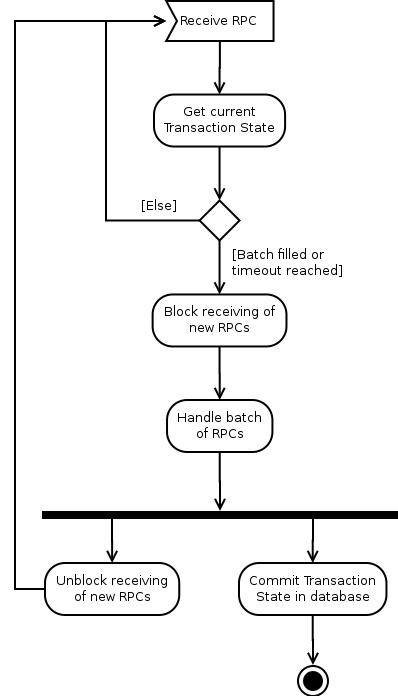
\includegraphics[scale=0.4]{resources/images/Implementation/rpc_batch_system_activity.png}
\caption{Activity diagram of RPC batching system}
\label{fig:impl_rpc_batch_system}
\end{figure}

At the beginning the TransactionStateManager service creates a
Transaction State object. Heartbeats start coming from the
ApplicationMasters and the NodeManagers in the form of RPCs. The
methods that are invoked, get the current TS from the
TransactionStateManager and piggyback them to the events
triggered, while various RM components handle those events in separate
threads.
The TransactionStateManager service keeps receiving RPCs
until a certain threshold of received RPCs -- default is 60, or until
a timeout has been reached -- default is 60 ms. At the point where
either of two is satisfied, it blocks responding to further
\texttt{getCurrentTransactionState} requests until all the RPCs in the
previous batch have been handled properly and put in the queue to be
committed in the database back-end. When this is done, it
creates a new Transaction State object and unblocks the receiving of
new RPCs. At the same time but in a \textbf{different thread}, the previous
Transaction State is committed to the database as described in Section
\ref{ssec:impl_aggr_mechanism}.

In Hops-YARN we have distributed the \emph{ResourceTrackingService} to
multiple machines in the cluster. They receive heartbeats from the
NodeManagers and persist them in NDB. MySQL Cluster has an event API
that can stream events to subscribers. In RM there is a custom C++
library that receives the events emitted from NDB, creates a Java
representation of them and put them in FIFO queue. In the background
there is a Hops service that polls from the queue and triggers the
appropriate events. The Transaction State is also included in these
events as the cascading modifications should be persisted in the
database. The same Transaction State manager service is used as
described in the previous paragraph, so from the manager's perspective
there is no difference between RPC events and NDB events.

\subsection{Aggregation mechanism}
\label{ssec:impl_aggr_mechanism}
Heartbeats arrive in the RM and invoke specific methods. The methods
invoked create specific events which include the TS and are sent to an
event dispatcher thread. The event dispatcher will forward the events
to the appropriate RM components that will trigger some actions and
probably create more events. All along the ``journey'' of these
events, TS track all the necessary modifications that should be
persisted in the database back-end. After all events in a batch have
been properly handled they should be committed in NDB.

Persisting in a non-volatile storage solution is expensive due to
exclusive locks, OS buffers, I/O interrupts etc. On top of that, if you are
persisting data in a remote database, then the network introduces
latency. For that reason, when a TS is ready to be committed, it forks
a new thread which will handle the actual database operations to
persist its state. Having the commit mechanism parallelized, multiple
TS can be persisted concurrently. At that point, we have just
invalidated our consistency model. Sooner or later we will
reach the case where two TS would be committed in the wrong order
corrupting the state of the database. The mechanism explained in
Section \ref{sssec:impl_aggr_old} controls the commit phase of each TS
guaranting that two conflicting TS will be committed in the correct
order. In Section \ref{sssec:impl_aggr_new} I will outline the
shortcomings of the existing mechanism and describe the new mechanism
I build that extends the previous.

\subsubsection{One TS per commit}
\label{sssec:impl_aggr_old}
The mechanism that controls the commit phase of TS should allow as
much as possible parallelism without violating our constraints. Our
constraints are:
\begin{itemize}
\item If the RPCs that are batched in Transaction State $TS_0$ have
  been fully handled before the RPCs batched in $TS_1$ and they both
  modify the same \textbf{YARN Application}, then the commit phase of $TS_0$
  should have been succefully completed \textbf{before} the commit
  phase of $TS_1$

\item If the RPCs that are batched in Transaction State $TS_0$ have
  been fully handled before the RPCs batched in $TS_1$ and they both
  modify the same \textbf{NodeManager}, then the commit phase of $TS_0$
  should have been succefully completed \textbf{before} the commit
  phase of $TS_1$

\item If Transaction States $TS_0$ and $TS_1$ modify different YARN
  Application \textbf{and} different NodeManager then they can be committed in parallel
\end{itemize}

Every TS keeps a list with the IDs of the applications it modifies and
a list with the IDs of the nodes it modifies. In the commit mechanism,
there is a FIFO queue for each and every application ID and node
ID. Before committing a TS, the mechanism puts it in the corresponding
queues both for the applications and the nodes it modifies. Then it
gets the IDs of the applications and nodes it modified. In order for
the TS to be committed, it should be in the \textbf{head} of the
queues for the corresponding application IDs \textbf{and} node IDs. If
it is not in the head of one application or node queue, it means that
a previous TS modified the same application or node and should be
committed before. The un-committed TS is put in a queue to be
examined later.

To make it more clear, I will give an example of how the commit mechanism
works. To make it easier, I assume that our only lock is on
application IDs and we have only three applications running. The FIFO
queues for the applications are depicted in Figure
\ref{fig:impl_tx_aggr_queue}. The initial state of the system is in
Figure \ref{fig:impl_tx_aggr_sub0} where no TS has been handled yet
and the queues are empty. Technically, the queues for the application
IDs and node IDs are created lazily when the TS has been fully handled
and is ready to be committed. RPCs for \texttt{TS\_0} have been
handled and is ready to be committed in the database. It modifies
entries for applications with ID \texttt{app\_0} and \texttt{app\_2},
so it is placed in the respective queues, Figure
\ref{fig:impl_tx_aggr_sub1}. \texttt{TS\_0} is the head
of the queues for the applications it modifies so it can start the
commit phase. Since a commit phase may fail and roll-back, it will be
removed from the queues when the transaction has been succefully
completed.

While \texttt{TS\_0} tries to persist its modifications to the
database, two more Transaction States have finished and are put in the
queue to be committed, Figure
\ref{fig:impl_tx_aggr_sub2}. \texttt{TS\_1} modifies applications
\texttt{app\_0} and \texttt{app\_1} while \texttt{TS\_2} modifies
applications \texttt{app\_1} and \texttt{app\_2}. The commit mechanism
checks whether \texttt{TS\_1} can be committed. Remember that
\texttt{TS\_0} is still committing to the database. The mechanism
fetches the applications that \texttt{TS\_1} modifies and checks if it
is the head in each queue. For \texttt{app\_1} it is in the head of
the queue but not for \texttt{app\_0}, \texttt{TS\_0} should finish
first. So it will be examined after \texttt{TS\_0} is done. The same
applies for \texttt{TS\_2}.

\texttt{TS\_0} is now complete and removed from the queues of the
applications it modified, Figure
\ref{fig:impl_tx_aggr_sub3}. \texttt{TS\_1} is now the head for
\texttt{app\_0} and \texttt{app\_1} so it starts the commit
phase. This is not the case though for \texttt{TS\_2} which still has
to wait for \texttt{TS\_1} to finish. \texttt{TS\_1} successfuly
completes its transaction, removed from the queues and now
\texttt{TS\_2} is in the head position, Figure
\ref{fig:impl_tx_aggr_sub4} so it can start committing to the database.

\begin{figure}
  \centering
  \begin{subfigure}[t]{0.3\textwidth}
    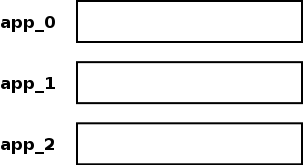
\includegraphics[scale=0.4]{resources/images/Implementation/commit_system_0.png}
    \caption{}
    \label{fig:impl_tx_aggr_sub0}
  \end{subfigure}
  \hfill
  \begin{subfigure}[t]{0.3\textwidth}
    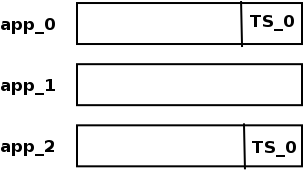
\includegraphics[scale=0.4]{resources/images/Implementation/commit_system_1.png}
    \caption{}
    \label{fig:impl_tx_aggr_sub1}
  \end{subfigure}
  \hfill
  \begin{subfigure}[t]{0.3\textwidth}
    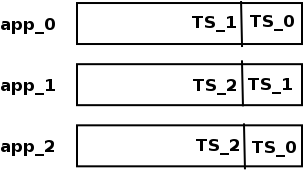
\includegraphics[scale=0.4]{resources/images/Implementation/commit_system_2.png}
    \caption{}
    \label{fig:impl_tx_aggr_sub2}
  \end{subfigure}
  \\[2em]
  \begin{subfigure}[t]{0.3\textwidth}
    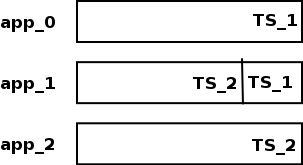
\includegraphics[scale=0.4]{resources/images/Implementation/commit_system_3.png}
    \caption{}
    \label{fig:impl_tx_aggr_sub3}
  \end{subfigure}
  \qquad
  \begin{subfigure}[t]{0.3\textwidth}
    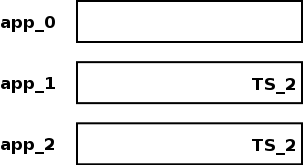
\includegraphics[scale=0.4]{resources/images/Implementation/commit_system_4.png}
    \caption{}
    \label{fig:impl_tx_aggr_sub4}
  \end{subfigure}

  \caption{Example of TS for the queue to be committed}
  \label{fig:impl_tx_aggr_queue}
\end{figure}

\subsubsection{Multiple TS per commit}
\label{sssec:impl_aggr_new}
The existing mechanism described in the section above provided the
consistency model that we required and parallelism for
non-conflicting TSs. The major issue that had to be addressed was that
for conflicting TSs $(1)$ they had to wait in the queue for another TS
to finish, in the example above \texttt{TS\_1} and \texttt{TS\_2} and
$(2)$ for every transaction committed we paid the network latency
penalty and the time probably to acquire locks etc. In order to solve
the first problem we examined different solutions. First I tried to
make a more fine-grained lock. Instead of locking on application and
node IDs, try to lock for containers. Although this solution whould
increase parallelism, it was very risky that we would end-up with a
corrupted state. Next solution was to remove the system with the
queues and replace it with exclusive reentrant locks. The expected
result was to increase performance but at the end it was the same.

The solution proposed in this section and implemented reduces both the
wait time in the queue for a TS to be committed and the RTT for each
transaction performed. The mechanism extends the method described in
Section \ref{sssec:impl_aggr_old} by aggregating multiple TSs into a
single one while it guarantees consistency. The queue system still
gives us the proper order in which the TSs should be persisted. A TSs
is examined if it should be persisted in the database. If it is not
possible to be persisted due to conflicting TSs then it is put in a
\emph{toBeAggregated} set. If it is permitted to commit, then it does so
and construct an extended TS called
\emph{AggregatedTransactionState}.

The \emph{AggregatedTransactionState} contains TSs from the
\emph{toBeAggregated} set that are eligible for commit according to the
following aggregation rules:
\begin{enumerate}
  \item A TS was not the head in its respective queues at the time it
    was examined for commit, but until now the conflicting TS(s) have
    been committed and removed. So now it is in the head of the
    queues.

  \item A TS is still not in the head of the queues, but the
    conflicting TSs that should be committed before, have been already
    aggregated in the \emph{AggregatedTransactionState}.
\end{enumerate}

The first case is trivial and we have examined it in the previous
section. For the second case, the mechanism gets the modified
application and node IDs from a Transaction State \texttt{TS\_a}.
Then it retrieves all the conflicting TSs from the appropriate queues
that are blocking \texttt{TS\_a} from being committed. If all of the
conflicting TSs have already been aggregated -- put in the
\emph{AggregatedTransactionState}, then the mechanism aggregates
\texttt{TS\_a} as well and it proceeds by examining the next TS in the
\emph{toBeAggregated} set. At the end of this process we will end-up
with a ``big'' Transaction State, the
\emph{AggregatedTransactionState} that will be committed in the
database. The \emph{AggregatedTransactionState} class actually extends
the \emph{TransactionState} class and for every TS that is aggregated
it updates the data structures with the modifications of the TS. The
\emph{toBeAggregated} data structure is a FIFO queue so the TSs that
are examined for aggregation are kept in the correct order. At the
end of the aggregation process, the data structures of the
AggregatedTransactionState hold the correct, most recent modifications to be persisted.

Consider the state of the queues as in Figure
\ref{fig:impl_tx_aggr_sub2}. Both \texttt{TS\_1} and \texttt{TS\_2}
cannot be committed because they are blocked by \texttt{TS\_0} so they
are added to the \emph{toBeAggregated} queue. At some
point \texttt{TS\_0} is committed in the database, removed from the
queues as in Figure \ref{fig:impl_tx_aggr_sub3}, creates the
\emph{AggregatedTransactionState} (ATS)
and starts the aggregation process. \texttt{TS\_1} is the first
candidate for aggregation. At that point \texttt{TS\_1} is at the head
of its respective queues and following the aggregation rule $1$ it is
aggregated. All the data structures of \texttt{TS\_1} are copied to
the data structures of the ATS. Next in the \emph{toBeAggregated} set
is \texttt{TS\_2}. \texttt{TS\_2} is not the head in the queue for
application \texttt{app\_1} but the conflicting TS, \texttt{TS\_1} has
already been aggregated. So according to aggregation rule $2$,
\texttt{TS\_2} is also aggregated, probably updating the values that
\texttt{TS\_1} has put in TSA. The \emph{toBeAggregated} set is now
empty and the ``big'' AggregatedTransactionState is committed to the
database. Compared to the existing commit mechanism, where we have
done three commits in the database, we have now reduced it to two.

\begin{figure}
\centering
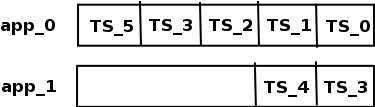
\includegraphics[scale=0.5]{resources/images/Implementation/commit_system_aggr_example.png}
\caption{Aggregate commit mechanism example}
\label{fig:impl_tx_aggr_example}
\end{figure}

Another example that demonstrates the improvement we have achieved is
described in the following paragraph. Consider the locking queues as
depicted in Figure \ref{fig:impl_tx_aggr_example} for two applications. All the Transaction
States are blocked behind \texttt{TS\_0} which is at the commit
phase. At that time the \emph{toBeAggregated} set contains
\texttt{TS\_1}-\texttt{TS\_5}. \texttt{TS\_0} finishes its commit phase, removes
itself from the locking queues and begins the aggregation phase. First
it examines \texttt{TS\_1}. It is in the head of the queue for
application \texttt{app\_0} and according to aggregation rule $1$ it
should be aggregated. Next in the \emph{toBeAggregated} set is
\texttt{TS\_2}. The conflicting state is \texttt{TS\_1}, which is
already aggregated so according to aggregation rule $2$ it is
aggregated too. \texttt{TS\_3} is in the head of the queue for
\texttt{app\_1} and all the conflicting TSs for \texttt{app\_0} have
been aggregated so it is also put in the
\emph{AggregatedTransactionState}. Similarly, \texttt{TS\_4} and
\texttt{TS\_5} are also aggregated. Now the
\emph{AggregatedTransactionState} contains the modifications of
\texttt{TS\_1}, \texttt{TS\_2}, \texttt{TS\_3}, \texttt{TS\_4},
\texttt{TS\_5} and begins the commit phase. With the previous commit
mechanism, every TS would have performed the commit phase individually introducing
considerable delay due to the RTT to the database, whereas with the
new commit mechanism we only require two commits in the database.

Aggregating several TSs into a single one introduced some erroneous
behaviour. NDB is very performant with transactions of small size but
the aggregation mechanism was overloading the transaction and NDB was
throwing errors. In order to mitigate this issue a TCP-like aggregation control
was put in place. In the beginning, the mechanism starts to aggregate
a small number of TSs. When the commit phase for that
\emph{AggregatedTransactionState} is successfully completed, the limit
is increased by some delta. It continues to increase until an error
message is received from the database. The transaction is rolled-back,
the limit for the number of aggregations is set to minimum and the
mechanism tries again to aggregate. Users can implement their own
policy as it fits their needs without having to change the commit
mechanism code.

Overall, the new commit mechanism addresses both the waiting time in
the queue and the communication latency. TSs do not have to wait in
the queue for all the conflicting TSs to be committed. Once one
conflicting TS is committed then the mechanism aggregates as many as
possible TSs. Moreover, since multiple TSs are squashed into a single
one, there is only one commit phase reducing a lot the network latency.
